\documentclass{ximera}

\input{../preamble.tex}


\title[Dig-In:]{The Second Fundamental Theorem of Calculus}

\begin{document}
\begin{abstract}
The accumulation of a rate is given by the change in the amount.
\end{abstract}
\maketitle




There is a another common form of the Fundamental Theorem of Calculus:

\begin{theorem}[Second Fundamental Theorem of Calculus]\index{Second Fundamental Theorem of Calculus}
  Let $f$ be continuous on $[a,b]$. If $F$ is \textbf{any}
  antiderivative of $f$, then
  \[
  \int_a^b f(x)\d x = F(b)-F(a).
  \]
  \begin{explanation}
    Let $a\le c\le b$ and write
    \begin{align*}
      \int_a^b f(x) \d x &= \int_a^c f(x) \d x + \int_c^b f(x) \d x \\
      &= \int_c^b f(x) \d x - \int_c^a f(x) \d x.
    \end{align*}
    By the First Fundamental Theorem of Calculus, we have
    \[
    F(b) = \int_c^b f(x) \d x\qquad\text{and}\qquad F(a) = \int_c^a f(x) \d x
    \] 
    for some antiderivative $F$ of $f$. So
    \[
    \int_a^b f(x) \d x = F(b)-F(a)
    \]
    for this antiderivative. However, \textbf{any} antiderivative
    could have be chosen, as antiderivatives of a given function
    differ only by a constant, and this constant \textit{always}
    cancels out of the expression when evaluating $F(b)-F(a)$.
\end{explanation}
\end{theorem}

From this you should see that the two versions of the Fundamental
Theorem are very closely related. In reality, the two forms are
\textbf{equivalent}, just differently stated. Hence people often
simply call them both ``The Fundamental Theorem of Calculus.''
One way of thinking about the Second Fundamental Theorem of Calculus is:
\begin{image}
  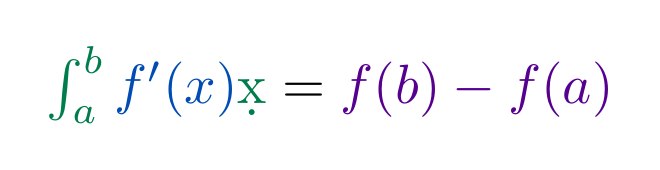
\begin{tikzpicture}[scale=2,every node/.style={transform shape}]
    \node at (0,0) {
      $\color{green!70!black!70!blue}\int_a^b\color{blue!70!green}f'(x)\color{green!70!black!70!blue}\d x\color{black} = 
      \color{purple!50!blue!90!black}f(b) - f(a)$
      };
  \end{tikzpicture}
\end{image}
This could be read as:%%BADBAD I want this all in bold and with colors
\begin{quote}\large\textbf{The \textcolor{green!70!black!70!blue}{accumulation} of a \textcolor{blue!70!green}{rate} is given by the \textcolor{purple!50!blue!90!black}{change in the amount}.}
\end{quote}


When we compute a definite integral, we first find an antiderivative
and then evaluate at the limits of integration. It is convenient to
first display the antiderivative and then evaluate.  A special
notation is often used in the process of evaluating definite integrals
using the Fundamental Theorem of Calculus. Instead of explicitly
writing $F(b)-F(a)$, we often write
\[
\eval{F(x)}_a^b
\]
meaning that one should evaluate $F(x)$ at $b$ and then subtract
$F(x)$ evaluated at $a$
\[
\eval{F(x)}_a^b = F(b)-F(a).
\]

Let's see some examples of the fundamental theorem in action.

\begin{example}
  Compute:
  \[
  \int_{-2}^2 x^3\d x
  \]
  \begin{explanation}
    We start by finding an antiderivative of $x^3$.  A correct choice
    is $\frac{x^{4}}{4}$, one could verify this by taking the
    derivative. Hence
    \begin{align*}
      \int_{-2}^2 x^3 \d x &=\eval{\frac{x^4}{4}}_{-2}^2\\
      &= \frac{2^4}{4} - \frac{(-2)^4}{4}\\
      &= 0.
    \end{align*}
  \end{explanation}
\end{example}



\begin{example}
  Compute:
  \[
  \int_0^5 e^t\d t
  \]
  \begin{explanation}
    We start by finding an antiderivative of $e^t$.  A correct choice
    is $\answer[given]{e^t}$, one could verify this by taking the
    derivative. Hence
    \begin{align*}
      \int_0^5 e^t \d t &= \eval{e^t}_0^5 \\
      &= e^5-\answer[given]{e^0}\\
      &= e^5-\answer[given]{1}.
    \end{align*}
  \end{explanation}
\end{example}


\begin{example}
Compute:
\[
\int_1^2\left(x^9 + \frac{1}{x}\right) \d x
\]
\begin{explanation}
We start by finding an antiderivative of $x^9 + \frac{1}{x}$.  A
correct choice is $\frac{x^{10}}{10} + \ln(x)$, one could verify this
by taking the derivative. Hence
\begin{align*}
\int_1^2\left(x^9 + \frac{1}{x}\right) \d x &= \eval{\frac{x^{10}}{10} + \ln(x)}_1^2 \\
&= \frac{2^{10}}{10} + \ln(2) - \answer[given]{\frac{1}{10}}.
\end{align*}
\end{explanation}
\end{example}







Now we know that to solve certain kinds of problems, those that
involve accumulation of some form, we ``merely'' find an
antiderivative and substitute two values and subtract. Unfortunately,
finding antiderivatives can be quite difficult. While there are a
small number of rules that allow us to compute the derivative of any
common function, there are no such rules for antiderivatives. There
are some techniques that frequently prove useful, but we will never be
able to reduce the problem to a completely mechanical process.







\end{document}
